\documentclass[a4paper,10pt]{article} %twocolumn
\usepackage[utf8]{inputenc} % letras acentuadas
\usepackage[portuguese]{babel} % tradução de títulos
\usepackage{algorithm} % ambiente para índice de algoritmos
\usepackage{algpseudocode} % fonte e estilo do algoritmo
\usepackage{tikz} % circuitos e automata
\usepackage{amsmath} % simbolos matematicos
\usepackage{graphicx} % inserir figuras
%[noend]

\usetikzlibrary{automata,positioning}

\floatname{algorithm}{Algoritmo} % tradução da palavra algorítimo no ambiente de índice

\title{O algoritmo de conversão de Autômato Finito Não-Determinístico - AFND para Expressão Regular - ER}
\author{Eduardo Couto Dinarte,\\ Iago Gade Gusmao Carrazzoni,\\ Lucca Maciel de Moraes}

\begin{document}

\maketitle

\begin{abstract}

Este artigo consiste na apresenta\c{c}\~{a}o e explica\c{c}\~{a}o de um algoritmo para converter um aut\^{o}mato finito n\~{a}o determin\'{i}stico num aut\^{o}mato finito determin\'{i}stico e, por fim, converter este numa express\~{a}o regular. O m\'{e}todo consiste em apresentar a teoria com imagens dos tr\^{e}s estados da convers\~{a}o seguida de um exemplo pr\'{a}tico. O objetivo deste texto \'{e} fixar o conte\'{u}do de convers\~{a}o de aut\^{o}matos e familiarizar os autores com a produ\c{c}\~{a}o de artigos cient\'{i}ficos utilizando a linguagem Latex.

\end{abstract}

\newpage
\section{Introdução aos Autômatos}

Um autômato é uma máquina abstrata que deve operar entre estados previamente definidos. É um modelo matemático utilizado para representar programas ou circuitos lógicos. É bem definido por uma quíntupla, cujos elementos são:
    \begin{itemize}
        \item Conjunto de estados (K);
        \item Alfabeto (A);
        \item Estado inicial (S);
        \item Conjunto de estados finais (F);
        \item Função de transição (ou função delta).
    \end{itemize}

A função de transição, por sua vez, é representada por uma tripla ordenada, onde os elementos são:
    \begin{itemize}
        \item Estado inicial;
        \item Transição;
        \item Estado final;
    \end{itemize}

\newpage
\section{Introdução ao Autômato Finito Não-Determinístico - AFND}

Aut\^{o}mato finito n\~{a}o determin\'{i}stico \'{e} aquele em que, em algum momento, n\~{a}o se tem certeza de qual \'{e} o estado atual, ou seja, \'{e} aquele que tem a palavra vazia ligando algum de seus estados. Segue um exemplo a seguir:

\begin{center}
\begin{tikzpicture}[shorten >=1pt,node distance=2cm,on grid,auto] 
   \node[state,initial] (q_0)   {$q_0$}; 
   \node[state] (q_1) [above right=of q_0] {$q_1$}; 
   \node[state] (q_2) [below right=of q_0] {$q_2$}; 
   \node[state,accepting](q_3) [below right=of q_1] {$q_3$};
   \node[state, accepting] (q_4) [right=of q_3] {$q_4$};
   \path[->]
       (q_0) edge node {$\epsilon$} (q_1)
             edge node [swap] {$\epsilon$} (q_2)
       (q_1) edge node {1} (q_3)
             edge [loop above] node {0} ()
       (q_2) edge node [swap] {0} (q_3)
             edge [loop below] node {1} ()
       (q_3) edge node {$\epsilon$} (q_4);
\end{tikzpicture}
\end{center}

\newpage
\section{Introdução ao Autômato Finito Determinístico - AFD}

Autômato finito determinístico é aquele em que se sabe exatamente qual o estado atual, ou seja, é aquele que não tem estados simultâneos (estados ligados por palavras vazias).
    \begin{center}
    \begin{tikzpicture}[shorten >=1pt,node distance=2cm,on grid,auto] 
        \node[state,initial] (q_0) {$q_0$};
        \node[state] (q_1) [above right=of q_0] {$q_1$};
        \node[state, accepting] (q_2) [right=of q_0] {$q_2$};
        \node[state] (q_3) [below right=of q_0] {$q_3$};
        \node[state] (q_4) [right=of q_1] {$q_4$};
        \node[state] (q_5) [below right=of q_2] {$q_5$};
        \node[state, accepting] (q_6) [below right=of q_4] {$q_6$};
        \path[->]
            (q_0) edge node {a} (q_1)
                  edge node {b} (q_2)
                  edge node {c} (q_3)
            (q_1) edge [loop above] node {a} ()
                  edge node {b} (q_4)
            (q_2) edge [loop above] node {c} ()
                  edge node {a} (q_4)
                  edge node {b} (q_5)
            (q_3) edge [loop below] node {b} ()
                  edge node {a} (q_5)
            (q_4) edge node {c} (q_6)
            (q_5) edge node {c} (q_6);
\end{tikzpicture}
\end{center}

\newpage
\section{Introdução à Expressão Regular - ER}

Expressão regular é uma cadeia de caracteres que engloba todas as palavras aceitas pelo autômato. Um autômato reduzido a expressão regular possui apenas um estado inicial e um estado final, ligados pela expressão regular.
\begin{center}
\begin{tikzpicture}[shorten >=1pt,node distance=2cm,on grid,auto] 
    \node[state,initial] (q_0) {$q_0$};
    \node[state,accepting] [below right=of q_0] (q_1) {$q_1$};
    \path[->]
        (q_0) edge node {aa*(b {$\lor$} c)*} (q_1);
\end{tikzpicture}
\end{center}

No tipo citado, é comum a aparição do caractere {$\lor$}, assim como o parêntese. Este se aplica da mesma forma que na matemática. Aquele é o conectivo lógico 'ou', que se aplica da mesma forma que na lógica.\\\\Também é comum a aparição do caractere '*' na expressão regular. Ele se chama estrela de Kleene, e denota zero ou mais repetições do caractere ( ou cadeia de caracteres ) ao qual foi aplicado.\\\\No exemplo acima, a estrela de Kleene foi aplicada ao caractere 'a' e à expressão (b {$\lor$} c). Neste, quer dizer que zero ou mais repetições da cadeia denotada serão aceitas, enquanto naquele, zero ou mais repetições do caractere denotado serão aceitos.

\newpage
\section{Conversão de AFND para AFD}

Para essa conversão, é utilizado o Algoritmo de Conversão de um Autômato Finito Não-determinístico (AFND) em um Autômato Finito Determinístico, que consiste em:
    \begin{itemize}
        \item Identificar os estados simultâneos do AFND;
        \item Identificar o estado inicial P0, o qual seu conjunto possui apenas o estado inicial da AFND;
        \item Aplicar em P0 a leitura de todo o alfabeto. O conjunto novo será composto pelo lugar da chegada;
        \item Identificar os estados resultantes;
        \item Para cada estado resultante criado, aplica-se o alfabeto;
        \item Repetir o procedimento até que não existam mais estados novos;
        \item Identificar os estados finais, que serão aqueles estados que possuírem os estados finais da AFND;     
        \item Montar a quíntupla do AFD;     
        \item Por fim, esboçar o grafo.    
    \end{itemize}

Para exemplificar, será realizada a conversão do AFND a seguir, cuja quíntupla é:\\K = \{0, 1, 2, 3, 4, 5\}\\A = \{a, b, c\}\\S = \{0\}\\F = \{3, 4\}\\D =\\(0, {$\epsilon$}, 1),\\(0, {$\epsilon$}, 2),\\(1, b, 3)\\(1, a, 5),\\(2, a, 5)\\(3, a, 3),\\(3, c, 4),\\(5, c, 5),\\(5, b, 4). \\
    \begin{center}
        \begin{tikzpicture}[shorten >=1pt,node distance=2cm,on grid,auto] 
            \node[state,initial] (q_0) {$q_0$};
            \node[state] [above right=of q_0](q_1) {$q_1$};
            \node[state] [below right=of q_0] (q_2) {$q_2$};
            \node[state,accepting] [right=of q_1] (q_3) {$q_3$};
            \node[state,accepting] [above right=of q_5] (q_4) {$q_4$};
            \node[state] [right=of q_2] (q_5) {$q_5$};
            \path[->]
                (q_0) edge node {$\epsilon$} (q_1)
                      edge node {$\epsilon$} (q_2)
                (q_1) edge node {b} (q_3)
                      edge node {a} (q_5)
                (q_2) edge node {a} (q_5)
                (q_3) edge [loop above] node {a} ()
                      edge node {c} (q_4)
                (q_5) edge [loop below] node {c} ()
                      edge node {b} (q_4);
        \end{tikzpicture}
    \end{center}

Daqui em diante as seguintes notações serão usadas:
    \begin{itemize}
        \item E(x): denota o conjunto de estados simultâneos a x;
        \item P(x): denota um estado maior, que engloba vários outros;
        \item D(P(x), A): denota a função delta de P(x) aplicando o alfabeto.
    \end{itemize}
    
Seguindo o algoritmo, o procedimento será o seguinte:
    \begin{itemize}
        \item Identificar os estados simultâneos do AFND:
            \\E(0) = \{0, 1, 2\}\\E(1) = \{1\}\\E(2) = \{2\}\\E(3) = \{3\}\\E(4) = \{4\}\\E(5) = \{5\}
        \item identificar o estado inicial P0, o qual seu conjunto possui o estado inicial da AFND:
            \\P(0) = E(0) = \{0, 1, 2\}
        \item aplicar em P0 a leitura de todo o alfabeto. O conjunto novo será composto pelo lugar da chegada:
            \\D(P(0), a) = (1, a, 5) U (2, a, 5) = E(5) U E(5) = \{5\}\\D(P(0), b) = (1, b, 3) = E(3) = \{3\}\\D(P(0), c) = vazio
        \item Identificar os estados resultantes:
            \\P(1) = D(P(0), a) = E(5) = \{5\}\\P(2) = D(P(0), b) = E(3) = \{3\}
        \item para cada estado resultante criado, aplica-se o alfabeto:
            \\D(P(1), a) = vazio\\D(P(1), b) = (5, b, 4) = E(4) = \{4\}\\D(P(1), c) = (5, c, 5) = E(5) = \{5\}
            \\D(P(2), a) = (3, a, 3) = E(3) = \{3\}\\D(P(2), b) = vazio\\D(P(2), c) = (3, c, 4) = E(4) = \{4\}
        \item repetir o procedimento até que não existam mais estados novos:
            \\D(P(1), b) = P(3) = E(4) = \{4\}\\D(P(1), c) = P(1) = E(1) = \{1\}\\D(P(2), a) = P(2) = E(2) = \{2\}\\D(P(2), c) = P(3) = \{4\}\\
            \\D(P(3), a) = vazio\\D(P(3), b) = vazio\\D(P(3), c) = vazio
        \item identificar os estados finais, que serão aqueles estados que possuírem os estados finais do AFND:
            \\F = {P(1), P(3)}
        \item montar a quíntupla do AFD:
            \\K = \{P(0), P(1), P(2), P(3)\}\\A = \{a, b, c\}\\S = \{P(0)\}\\F = \{P(2), P(3)\}\\Pode ser difícil observar os elementos da função delta. Eles serão todos os D(P(x), 'caractere') que calculamos. Assim:\\D =\\(P0, a, P1),\\(P0, b, P2),\\(P1, b, P3),\\(P1, c, P1),\\(P2, a, P2),\\(P2, c, P3).
    \end{itemize}
    \begin{center}
        \begin{tikzpicture}[shorten >=1pt,node distance=2cm,on grid,auto] 
            \node[state,initial] (P_0) {$P_0$};
            \node[state] [above right=of P_0] (P_1) {$P_1$};
            \node[state] [below right=of P_0] (P_2) {$P_2$};
            \node[state,accepting] [below right=of P_1] (P_3) {$P_3$};
            \path[->]
                (P_0) edge node {a} (P_1)
                      edge node {b} (P_2)
                (P_1) edge [loop above] node {c} ()
                      edge node {b} (P_3)
                (P_2) edge [loop below] node {a} ()
                      edge node {c} (P_3);
        \end{tikzpicture}
    \end{center}

\newpage
\section{Conversão AFD - ER}
    Nessa conversão, o número de transições que o estado inicial possui será muito importante: a ER será uma composição das expressões obtidas seguindo cada um dos caminhos a partir do estado inicial. Por exemplo, se o estado inicial possui três transições para outros estados, a ER será uma composição de três expressões, separadas, na ER final, pelo conectivo lógico 'OU'. Em suma, se há três caminhos, é possível seguir pelo primeiro OU pelo segundo OU pelo terceiro. Essa lógica se mantém na ER. Esclarecida esta questão, inicia-se o algoritmo.
    \begin{itemize}
        \item Identificar a quantidade de transições do estado inicial.\\Nº de transições do estado inicial: 2.
        \item Criar dois outros estados. Um estará ligado aos estados finais do autômato por uma palavra vazia, enquanto o outro estará ligado ao estado inicial pela mesma. Aquele ligado ao estado inicial passará a ser o novo estado inicial, enquanto o ligado aos estados finais, passará a ser o estado final. Eles serão os únicos existentes na ER.
            \begin{center}
                \begin{tikzpicture}[shorten >=1pt,node distance=2cm,on grid,auto] 
                    \node[state] (P_0) {$P_0$};
                    \node[state] [above right=of P_0] (P_1) {$P_1$};
                    \node[state] [below right=of P_0] (P_2) {$P_2$};
                    \node[state,accepting] [below right=of P_1] (P_3) {$P_3$};
                    \node[state,initial] [above left=of P_0] (P_4) {$P_4$};
                    \node[state,accepting] [below right=of P_3] (P_5) {$P_5$};
                    \path[->]
                        (P_0) edge node {a} (P_1)
                              edge node {b} (P_2)
                        (P_1) edge [loop above] node {c} ()
                              edge node {b} (P_3)
                        (P_2) edge [loop below] node {a} ()
                              edge node {c} (P_3)
                        (P_3) edge node {$\epsilon$} (P_5)
                        (P_4) edge node {$\epsilon$} (P_0);
                \end{tikzpicture}
            \end{center}
        \item Colapsar estados até que só reste os dois criados. Consiste em retirar um estado, ligando o estado de chega nele ao estado no qual ele chega. A escolha do estado a se colapsar é completamente arbitrária.\\No exemplo, os primeiros estados a serem colapsados serão o P4 e o P2.\\A única transição nesses estados tem os mesmos como estado inicial e final. Portanto, é a mais simples situação a se considerar. Basta inserir A* na transição, onde A é um caractere qualquer.
        \begin{center}
            \begin{figure}[!htb]
                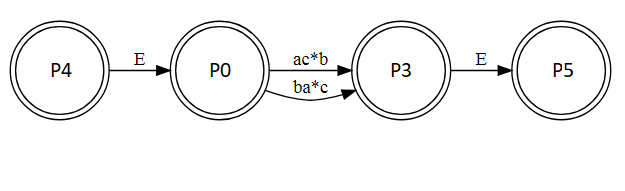
\includegraphics[scale = 1]{Figura_ex15.png}
            \end{figure}
        \end{center}
            %\graphicspath{{figuras/}}
            %\begin{document}
            %\begin{figure}[!htb]
            %    \centering
            %    \includegraphics{droopy}
            %    \caption{Legenda}
            %    \label{figRotulo}
            %\end{figure}

    \end{itemize}

\end{document}
